%%%%%%%%%%%%%%%%%%%%%%%%%%%%%%%%%%%%%%%%%%%%%%%%%%%%%%%%%%%%%%%%%%%%%
%
% VC36O Writeup Template
%
% This is a LaTeX document. LaTeX is a markup language for producing 
% documents. Your task is to fill out this
% document, then to compile this into a PDF document. 
% You will then upload this PDF to `Moodle'.
%
% 
% TO COMPILE:
% > pdflatex thisfile.tex
%
% For references to appear correctly instead of as '??', you must run 
% pdflatex twice.
%
% If you do not have LaTeX and need a LaTeX distribution:
% - Personal laptops (all common OS): www.latex-project.org/get/
%
% If you need help with LaTeX, please come to office hours. 
% Or, there is plenty of help online:
% https://en.wikibooks.org/wiki/LaTeX
%
% Good luck!
%
%%%%%%%%%%%%%%%%%%%%%%%%%%%%%%%%%%%%%%%%%%%%%%%%%%%%%%%%%%%%%%%%%%%%%
%
% How to include two graphics on the same line:
% 
% \includegraphics[\width=0.49\linewidth]{yourgraphic1.png}
% \includegraphics[\width=0.49\linewidth]{yourgraphic2.png}
%
% How to include equations:
%
% \begin{equation}
% y = mx+c
% \end{equation}
% 
%%%%%%%%%%%%%%%%%%%%%%%%%%%%%%%%%%%%%%%%%%%%%%%%%%%%%%%%%%%%%%%%%%%%%%%%%%%%%%%%%%%%%%%%%%%%%%%%

\documentclass[11pt]{article}

\usepackage[english]{babel}
\usepackage[utf8]{inputenc}
\usepackage[colorlinks = true,
            linkcolor = blue,
            urlcolor  = blue]{hyperref}
\usepackage[a4paper,margin=1.5in]{geometry}
\usepackage{stackengine,graphicx}
\usepackage{fancyhdr}
\setlength{\headheight}{15pt}
\usepackage{microtype}
\usepackage{times}
\usepackage{booktabs}

% From https://ctan.org/pkg/matlab-prettifier
\usepackage[numbered,framed]{matlab-prettifier}

\frenchspacing
\setlength{\parindent}{0cm} % Default is 15pt.
\setlength{\parskip}{0.3cm plus1mm minus1mm}

\pagestyle{fancy}
\fancyhf{}
\lhead{Project Writeup}
\rhead{VC36O 2018/1}
\rfoot{\thepage}

\date{}

\title{\vspace{-1cm}Project 2 Writeup}


\begin{document}
\maketitle
\vspace{-3cm}
\thispagestyle{fancy}

\section*{Instructions}
\begin{itemize}
  \item Describe any interesting decisions you made to write your algorithm.
  \item Show and discuss the results of your algorithm.
  \item Feel free to include code snippets, images, and equations.
  \item Use as many pages as you need, but err on the short side If you feel you only need to write a short amount to meet the brief, th
  
  \item \textbf{Please make this document anonymous.}
\end{itemize}

\section*{Introdução}

Neste trabalho ajustaremos a distribuição da intensidade do pixel em uma imagem, de modo que um histograma de um patch obtido coincida com o histograma de um patch extraído de outra imagem tirada de outra câmera posicionada de forma diferente e possivelmente com balanço de branco e brilho e contraste diferentes. Os patches devem ser da mesma região na cena e, portanto, devem ser transformados para corresponder a uma região retangular. Os patches e imagens inteiras serão fornecidos neste trabalho.


\section*{Implementação}

Como as especificações não ficaram bem definidas, outro método foi utilizado para a resolução deste trabalho, sendo o método a utilização de uma função de distribuição cumulativa.

Primeiramente é calculado a função de distribuição cumulativa de cada cor do histograma, sendo elas, vermelho, verde e azul. Após isso, pode haver um caso em que não exista exatamente uma igualdade entre cada histograma, então, é calculado a menor diferença absoluta entre os dois histogramas.



Foi utilizado o \textit{software} Octave\footnote{https://www.gnu.org/software/octave/} para a implementação do trabalho, o código comentado pode ser verificado logo abaixo: 

Código utilizado:
\begin{lstlisting}[style=Matlab-editor]
clear;
clc;

pkg load image

%carrega as imagens
img1 = imread('img1_patch.png');
img2 = imread('img2_patch.png');
img3 = imread('img2.png');

%tira o histograma de cada cor das 2 imagens_patch
img1red = imhist(img1(:,:,1));
img1green = imhist(img1(:,:,2));
img1blue = imhist(img1(:,:,3));

img2red = imhist(img2(:,:,1));
img2green = imhist(img2(:,:,2));
img2blue = imhist(img2(:,:,3));

%cria uma matriz de zeros para cada cor
Mred = zeros(256,1,'uint8');
Mgreen = zeros(256,1,'uint8');
Mblue = zeros(256,1,'uint8');

%calcula a funcao de distribuicao cumulativa para cada cor
cdf1red = cumsum(img1red) / numel(img1);
cdf2red = cumsum(img2red) / numel(img2);

cdf1green = cumsum(img1green) / numel(img1);
cdf2green = cumsum(img2green) / numel(img2);

cdf1blue = cumsum(img1blue) / numel(img1);
cdf2blue = cumsum(img2blue) / numel(img2);

%calcula um mapeamento que transforme uma intensidade da primeira
% imagem de modo que ela esteja de acordo com a distribuicao de
% intensidade da segunda imagem
for redidx = 1 : 256
    [~,redind] = min(abs(cdf2red(redidx) - cdf1red));%acha um valor aprox no vetor do histograma senao coloca o valor minimo
    Mred(redidx) = redind-1; %desconsidera o ultimo pq histograma da imagem vai de 0 a 255
end


for greenidx = 1 : 256
    [~,greenind] = min(abs(cdf2green(greenidx) - cdf1green));
    Mgreen(greenidx) = greenind-1;
end

for blueidx = 1 : 256
    [~,blueind] = min(abs(cdf2blue(blueidx) - cdf1blue));
    Mblue(blueidx) = blueind-1;
end

%Carrega cada cor na imagemfinal.
%Transforma em double pois img1 e do tipo uint8 e satura valores se voce tentar ir alem de 255
% para garantir que cheguemos a 256, devemos utilizar o tipo double. 
imgfinal(:,:,1) = Mred(double(img3(:,:,1))+1);
imgfinal(:,:,2) = Mgreen(double(img3(:,:,2))+1);
imgfinal(:,:,3) = Mblue(double(img3(:,:,3))+1);

%salva a imagem final
imwrite(imgfinal, "saida.png")

\end{lstlisting}

\section*{Resultados}

A figura \ref{fig:result1} mostra os resultados obtidos através da realização deste trabalho.

\begin{figure}[h]
    \centering
    \includegraphics[width=6cm]{img2.png}
    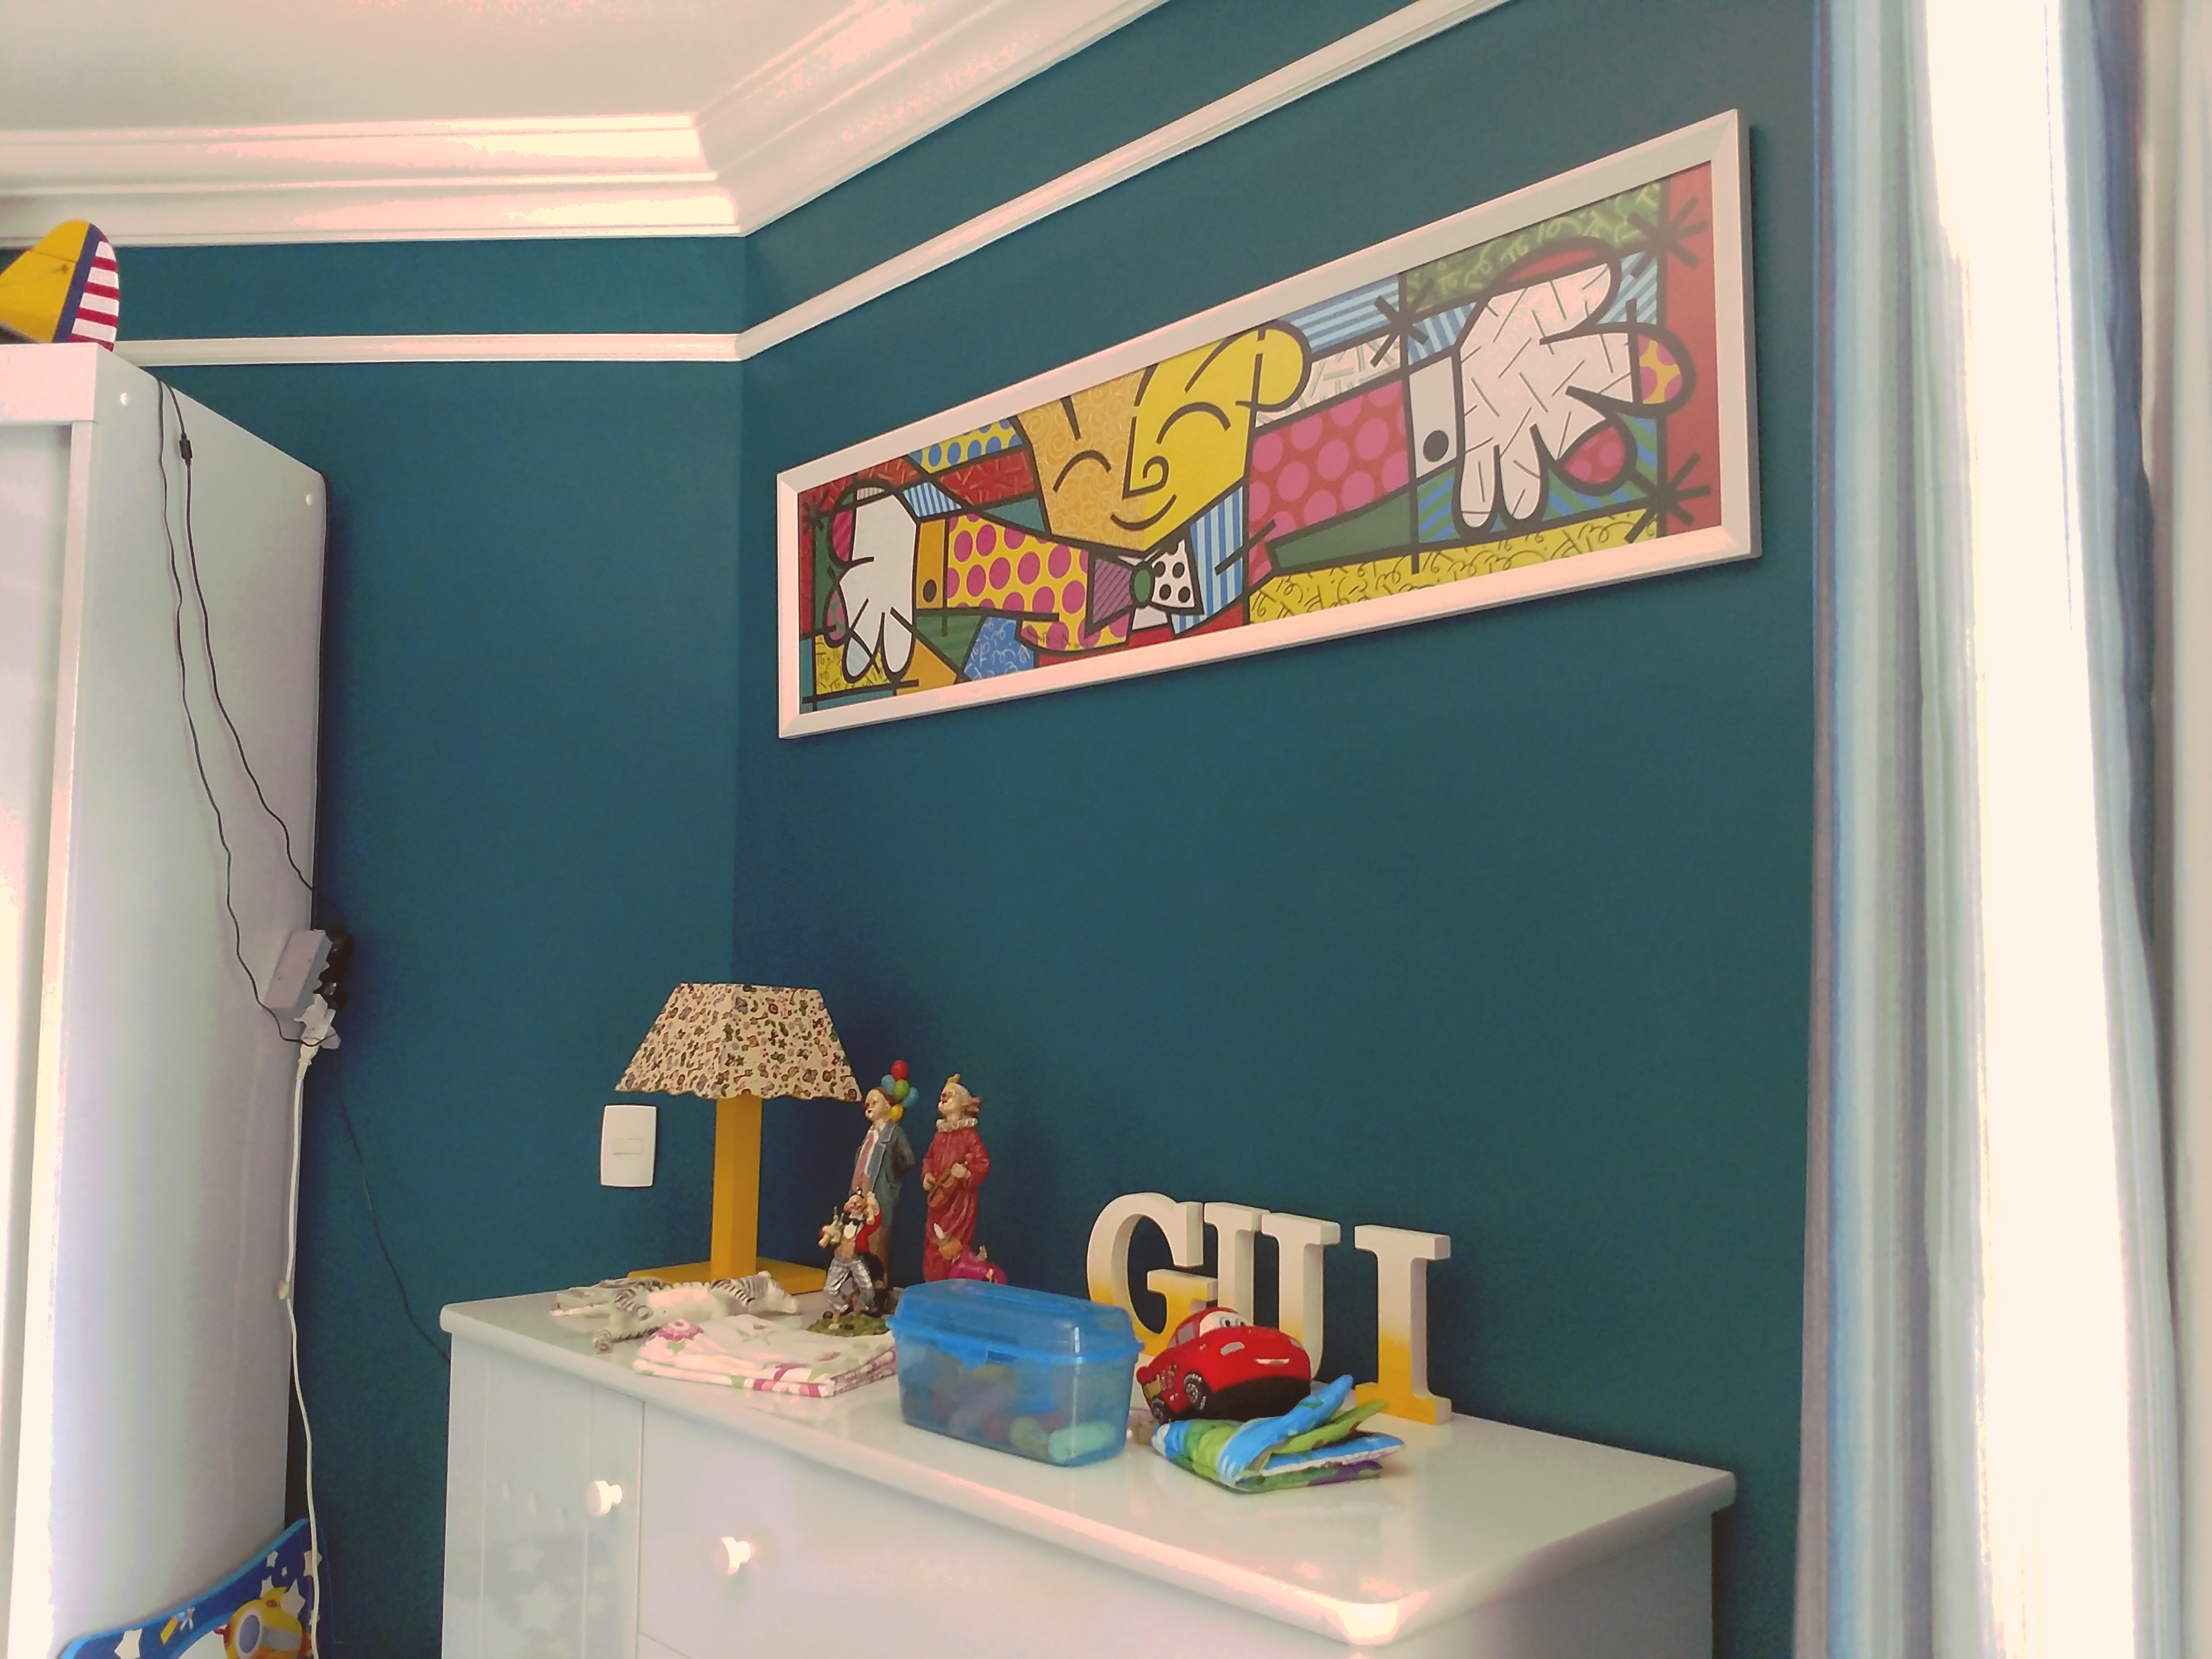
\includegraphics[width=6cm]{saida.png}
    \caption{\emph{Esquerda:} Imagem inicial. \emph{Direita:} Resultado obtido.}
    \label{fig:result1}
\end{figure}


\end{document}
